\documentclass[tikz]{standalone}


\usetikzlibrary{shapes, shapes.geometric, shapes.misc, shapes.arrows}
%\usetikzlibrary{3d, perspective}
\usetikzlibrary{arrows.meta}

\usetikzlibrary{shapes}
\usetikzlibrary{angles}
\usetikzlibrary{calc} 

\usetikzlibrary{positioning}
\usetikzlibrary{decorations.pathreplacing, decorations.markings, decorations.text, calligraphy}

\begin{document}

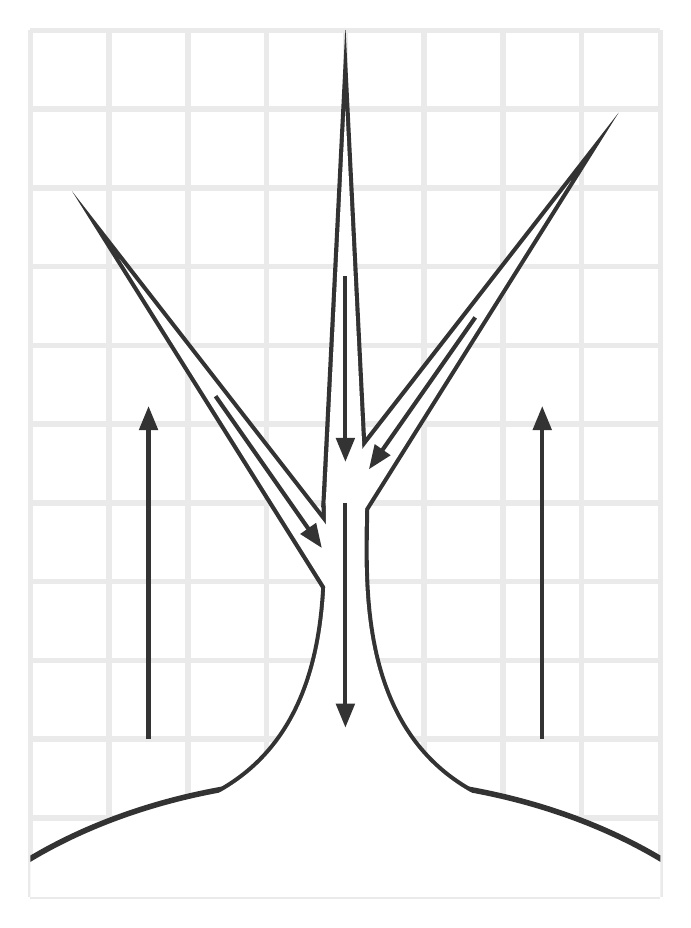
\begin{tikzpicture}[black!80, line width = 2pt]

    \def\Ybound{11}
    \def\Xbound{4}

    \draw[opacity = 0.1] (-\Xbound,-0) grid (\Xbound,\Ybound);
    \clip[use as bounding box] (-\Xbound,-0) rectangle (\Xbound,\Ybound);

    \def\nuclea{2}
    \def\radius{3}
    \def\angle{35}
    \def\angledos{3}
    \def\branchLen{5}

    \coordinate (O) at (0,-2.5);



    
    \path (O) -- (0,5) coordinate (Junc);
    \path foreach \SIGN/\PEAK/\STEM in {-/I/(Junc), \angle-/II/(Junc), +/III/(90:4)} 
        {\STEM -- ([turn]\SIGN \angle:\branchLen) coordinate (Top\PEAK) };

    \foreach \CENTER/\ANG in {TopI/-\angle, TopII/0, TopIII/+\angle}{
        \begin{scope}[shift = (\CENTER), rotate = \ANG]
            \draw[miter limit = 25, line width = 3pt] 
                {(-0.255,-\branchLen - 0.06) -- (\CENTER) -- (0.25,-\branchLen)};
        \end{scope}}
        
    \draw[line width = 3pt] ( 2.5, 1) .. controls ( 0, 1.5) and ( 0.25,4) .. ( 0.25,5);
    \draw[line width = 3pt] (-2.5, 1) .. controls (-0, 1.5) and (-0.25,4) .. (-0.25,5);


    \foreach \CENTER/\ANG in {TopI/-\angle, TopII/0, TopIII/+\angle}{
        \begin{scope}[shift = (\CENTER), rotate = \ANG]
            \fill[white, miter limit = 25] 
                {(-0.25,-\branchLen) -- (\CENTER) -- (0.25,-\branchLen)};
        \end{scope}}
    
    \begin{scope}[scale = 1, transform shape,fill = white]
        \filldraw[rounded corners]  
                (O) ellipse [x radius= 3*\nuclea , y radius= 2.0*\nuclea ];
    \end{scope}

    \fill[white, line width = 1pt] ( 2.5, 1) .. controls ( 0, 1.5) and ( 0.25,4) .. ( 0.25,5.04) -- (-0.25,5.04) .. controls (-0.25,4) and (-0, 1.5) .. (-2.5, 1) -- cycle;
    
    \foreach \CENTER/\STEM/\ANG in {TopI/(Junc)/-90-\angle, TopII/(Junc)/-90, TopIII/(90:4)/-90+\angle}{
            \path (\CENTER) -- \STEM node (Barrow) [pos = 0.85, fill, isosceles triangle, rotate = \ANG, minimum height = 3mm, inner sep = 1pt] {}; 
            \draw[line width = 1.5pt] ($(\CENTER)!0.5!(Barrow)$) -- ($(\CENTER)!1.02!(Barrow)$); 
        }

        
    \draw[line width = 1.5pt] (Junc) -- ($(Junc)!0.35!(O)$) node [fill, isosceles triangle, rotate = -90, minimum height = 3mm, inner sep = 1pt] {}; 

    \draw[line width = 1.5pt] foreach \SIGN in {+,-}{(\SIGN 2.5,2) -- +(0,4) node [fill, isosceles triangle, rotate = 90, minimum height = 3mm, inner sep = 1pt] {}};


\end{tikzpicture}

\end{document}